\documentclass{iyte}

% Caption Centering
% --------------
%\usepackage{caption}
 
%\captionsetup{justification=centering,singlelinecheck=false}

%\usepackage{graphicx}
\graphicspath{ {./images/} } 

% Using Hyperref
% --------------
%\usepackage[unicode]{hyperref}
%\hypersetup{
%	colorlinks   = true,    % Colours links instead of ugly boxes
%	urlcolor     = blue,    % Colour for external hyperlinks
%	linkcolor    = black,   % Colour of internal links; disabled for table of contents
%	citecolor    = black      % Colour of citations
%}

\usepackage{url}
\usepackage{natbib}
\usepackage{booktabs}
\usepackage{blindtext}
\usepackage{tabularx}
\usepackage{graphicx}
\usepackage{adjustbox}
\usepackage{amsmath,tikz-cd}
% \usepackage{fancyfoot}

\usepackage{caption}
\usepackage{subcaption}

\usepackage{titlesec}
\titlelabel{\thetitle.\quad}
\setlength{\bibhang}{1.27cm}

% Redefine the caption format for figures
\captionsetup[figure]{labelsep=period}

% Redefine the caption format for tables
\captionsetup[table]{labelsep=period}


\begin{document}
\pagenumbering{roman}

% --------------

% Title Page Definitions
\thesistitle{TRANSFORMERS USING LOCAL ATTENTION MAPPINGS FOR LONG TEXT DOCUMENT CLASSIFICATION}
\turkishthesistitle{UZUN METİN BELGESİ SINIFLANDIRMASI İÇİN YEREL DİKKAT HARİTALAMALARINI KULLANAN TRANSFORMATÖRLER}

\thesisauthor{Bekir Ufuk HAMAN}
\thesisdegree{MASTER OF SCIENCE}
\thesismajor{Computer Engineering}
\thesisdate{December}{2023}

% Add Title Page
%The MIT License (MIT) Ronny Majani
%
%Copyright (c) 2018
%
%Permission is hereby granted, free of charge, to any person obtaining a copy
%of this software and associated documentation files (the "Software"), to deal
%in the Software without restriction, including without limitation the rights
%to use, copy, modify, merge, publish, distribute, sublicense, and/or sell
%copies of the Software, and to permit persons to whom the Software is
%furnished to do so, subject to the following conditions:
%
%The above copyright notice and this permission notice shall be included in all
%copies or substantial portions of the Software.
%
%THE SOFTWARE IS PROVIDED "AS IS", WITHOUT WARRANTY OF ANY KIND, EXPRESS OR
%IMPLIED, INCLUDING BUT NOT LIMITED TO THE WARRANTIES OF MERCHANTABILITY,
%FITNESS FOR A PARTICULAR PURPOSE AND NONINFRINGEMENT. IN NO EVENT SHALL THE
%AUTHORS OR COPYRIGHT HOLDERS BE LIABLE FOR ANY CLAIM, DAMAGES OR OTHER
%LIABILITY, WHETHER IN AN ACTION OF CONTRACT, TORT OR OTHERWISE, ARISING FROM,
%OUT OF OR IN CONNECTION WITH THE SOFTWARE OR THE USE OR OTHER DEALINGS IN THE
%SOFTWARE.



\begin{titlepage}
	% Commands for positioning 'textbox' elements in the page
	\singlespacing
	\makeatletter
	\newcommand{\fromtop}[1]{%
		\dimexpr+\Gm@tmargin+#1\baselineskip\relax
	}
	\newcommand{\fromleft}[1]{%
		\dimexpr+\Gm@bindingoffset+\Gm@lmargin+#1\relax
	}
	\makeatother
	\newcommand{\textboxwidth}{\textwidth}
	\newcommand{\fromleftoffset}{\fromleft{0cm}}
	\newcommand*{\vsinglespaces}[1]{\singlespacing\vspace*{#1\baselineskip}}
	\setlength{\TPHorizModule}{\textwidth}
	\setlength{\TPVertModule}{\textwidth}
	% Commands for setting the fonts of this page
	\newcommand*{\titlefont}[1]{\onehalfspacing\textbf{\fontsize{18pt}{27pt}\selectfont{\strut#1\strut}}\singlespacing}
	\newcommand*{\subtitlefont}[1]{\onehalfspacing\textbf{\setstretch{0.75}\fontsize{14pt}{21pt}\selectfont#1}\singlespacing}
	% Title Page main content
	\begin{center}
		% Thesis Title
		\vsinglespaces{3}
		\titlefont{
			\showthesistitle
		}
		% Middle Block
		\begin{textblock*}{\textboxwidth}(\fromleftoffset,\fromtop{16})
			\subtitlefont{
				A Thesis Submitted to \\
				the Graduate School of Engineering and Sciences of\\
				\.{I}zmir Institute of Technology\\
				in Partial Fulfillment of the Requirements for the Degree of\linebreak\\
				\showthesisdegree\linebreak\\
				in \showthesismajor
			}

			\vsinglespaces{4}
			\subtitlefont{
				by\\
				\showthesisauthor
			}

			\vsinglespaces{7}
			\subtitlefont{\showthesisdate}
                \vspace{-0.45cm}
			\subtitlefont{  \.{I}ZM\.{I}R}
		\end{textblock*}

	\end{center}
	\onehalfspacing
\end{titlepage}
\addtocounter{page}{1}  % add 1 to the page counter (so Title page counts as page i)
\newpage

% --------------

% Signature Page Definitions
\signaturedate{7}{December}{2023}
\thesiscommitteememberA{Assoc. Prof. Selma TEK\.{I}R}{Computer Engineering}{İzmir Institute of Technology}
\thesiscommitteememberB{Assoc. Prof. Tolga AYAV}{Computer Engineering}{İzmir Institute of Technology}
\thesiscommitteememberC{Asst. Prof. Kaan KURTEL}{Software Engineering}{İzmir University of Economics}

\thesissupervisor{Assoc. Prof. Selma TEK\.{I}R}{Computer Engineering}{İzmir Institute of Technology}

% \thesiscosupervisor{Asst. Prof. XXXXXXXX}{Comp Eng}{IYTE}
\thesisheadofdepartment{Prof. Dr. Cüneyt F. \\BAZLAMA\c{C}CI}{Computer Engineering}
\thesisdeanofgraduateschool{Prof. Dr. Mehtap EANES}

% Uncomment to manually set the vertical spacing of the signature page
% \setsignaturepagespacing{0.8cm}  % replace the argument with the desired value

% Add Signature Page
\newgeometry{left=2.2cm, top=2.5cm,}
{\thispagestyle{empty}  % disable page numbering here
	We approve the thesis of \textbf{\showthesisauthor}\\
	
	\textbf{Examining Committee Members:}\\
	
	
	\ifdefined\showthesiscommitteememberA
		\showthesiscommitteememberA
	\fi
	
	\ifdefined\showthesiscommitteememberB
	\showthesiscommitteememberB
	\fi
	
	\ifdefined\showthesiscommitteememberC
	\showthesiscommitteememberC
	\fi
	
	\ifdefined\showthesiscommitteememberD
	\showthesiscommitteememberD
	\fi
	
	\ifdefined\showthesiscommitteememberE
	\showthesiscommitteememberE
	\fi
	
	\vspace{3em}
	\hfill
	\textbf{\showsignaturedate}
	\vspace{3ex}
	
	\showthesissupervisor\hfill
	\ifdefined\showthesiscosupervisor
	\showthesiscosupervisor
	\fi
	
	\showthesisheadofdepartment\hfill
	\showthesisdeanofgraduateschool
}
\restoregeometry

%\begin{minipage}{7cm}%
%	\vspace{1.0cm}\namesigdatehrule{7cm}\smallskip
%	\noindent{
%			Asst. Prof. Mustafa Özuysal\\
%			Department of Computer Engineering, Izmir Institute of Technology
%		}
%\end{minipage}
\newpage

% --------------

\begin{abstract}

Transformer models are powerful and flexible encoder-decoder structures that have proven their success in many fields, including natural language processing. Although they are especially successful in working with textual input, classifying texts, answering questions, and producing text, they have difficulty processing long texts. Current leading transformer models such as BERT limit input lengths to 512 tokens. The most prominent reason for this limitation is that the self-attention operation, which forms the backbone of the transformer structure, requires high processing power. This processing power requirement, which increases quadratically with the input length, makes it impossible for transformers to process long texts. However, new transformer structures that use various local attention mapping methods have begun to be proposed to overcome the text length challenge. This study first proposes two alternative local attention mapping methods to make transformer models capable of processing long texts. In addition, it presents the "Refined Patents" dataset consisting of 200,000 patent documents, specifically prepared for the long text document classification task. The proposed attention mapping methods, Term Frequency - Inverse Document Frequency (TF-IDF) and Point Mutual Information (PMI), create a sparse version of the self-attention matrix based on the occurrence statistics of words and word pairs. These methods were implemented based on the Longformer and Big Bird models, and tested on the Refined Patents dataset. Test results show that both proposed approaches are acceptable local attention mapping alternatives and can be used to enable long text processing in transformers.
\end{abstract}

\begin{ozet}

Transformatör modelleri doğal dil işleme dahil olmak üzere, pek çok alanda başarılarını kanıtlamış güçlü ve esnek kodlayıcı çözücü yapılarıdır. Özellikle metinsel girdilerle çalışmak, metinleri sınıflandırmak, soru cevaplamak, metin üretmek konusunda başarılı olsalar da uzun metinleri işlemekte zorlanırlar. BERT gibi mevcut önde gelen transformer modelleri, girdi uzunluklarını 512 kelime ile sınırlamıştır. Bu durumun en öne çıkan sebebi, transformatör yapısının bel kemiğini oluşturan öz dikkat operasyonunun yüksek işlem gücüne ihtiyaç duyuyor olmasıdır. Girdi uzunluğu ile karesel oranda artan bu işlem gücü ihtiyacı, transformerlar için uzun metinlerin işlenmesini imkansız hale getirmektedir. Ancak metin uzunluğu sorununun üstesinden gelmek için çeşitli yerel dikkat haritalandırma yöntemleri kullanan yeni transformatör yapıları önerilmeye başlanmıştır. Bu çalışma öncelikle transformatör modellerini uzun metinleri işleyebilir hale getirmek için iki alternatif lokal dikkat haritalandırması yöntemi önermektedir. Buna ek olarak, uzun metin sınıflandırma görevi için özel olarak hazırlamış ve 200.000 patent dokümanından oluşan "Refined Patents" verisetini sunar. Önerilen dikkat haritalandırması yöntemleri, Terim Frekansı - Tersine Doküman Frekansı (TF-IDF) ve Noktasal Karşılıklı Bilgi (PMI), kelime ve kelime çiftlerinin görülme istatistiklerinden yola çıkarak öz dikkat matrisinin seyrek halini oluşturarak transformatör modellerinin uzun metinleri işleyebilmesine olanak sağlar. Bu yöntemler, türünün öncü örneklerinden Longformer ve Big Bird modelleri temel alınarak uygulanmış ve Refined Patents veriseti üzerinde üzerinde test edilmiştir. Test sonuçları önerilen iki yaklaşımın da kabul edilebilir lokal dikkat haritalandırması alternatifi olduklarını ve transformatörlerde uzun metin işlenmesini mümkün kılmak için kullanılabileceklerini göstermektedir.
\end{ozet}

\tableofcontents
\newpage
\listoffigures
\newpage
\listoftables
\newpage


\chapter{INTRODUCTION}
\pagenumbering{arabic}

Transformers are encoder-decoder structures that have gained a place in natural language processing and many areas of machine learning. They have proven their robustness and success in various tasks and have reached high popularity shortly after their introduction due to their relatively simple structure and immense success in natural language processing tasks. In addition to usages such as text generation, summarization, and question answering, text classification has also become one of the main usage areas of transformers and has been operated in a wide range of applications, from topic-based classification tasks to sentiment analysis. However, while their recognizable success results in several state-of-the-art results for natural language processing tasks, there are also issues where transformers, with an attention mechanism forming their basis, face bottlenecks that impose strict limitations on them.

The ability of transformers to quickly process large-scale natural language corpora and to have a high understanding and processing capacity on this sequential data is primarily due to a fundamental structure called the attention mechanism. However, this very structure also constitutes their weak point. The attention mechanism, a parallel process whose basis can be summarized as projecting linear transformations of the word embeddings to matrix multiplication, resulting in attention matrix values, is designed to process the input of the transformer in a single cycle. Although this structure gives the transformer its signature speed and influence advantage over a serialized approach when working on short texts, as the length of the text input increases, the amount of required memory the transformer needs to operate also increases.

The dot product of two weight matrices, which are different versions of the same input embeddings, requires a computation power equal to the square of the input size that assembles the matrices. Meaning the computational complexity of the self-attention mechanism is proportional to the square of the input size. In other words, there is a quadratic relationship between input size and the complexity. Therefore, increasing the input size beyond a certain amount increases this self-attention mechanism's complexity to unmanageable levels.

One of the critical areas where this problematic case occurs is the document classification task, which is a text classification sub-task that requires processing longer and structured texts. In particular, as \cite{ETC} experimentally shows, the transformers under-perform for the task of long document classification compared to a similar task with shorter texts. However, document classification is a critical process that can be used by all kinds of businesses, from government offices to libraries and corporate companies to patent offices, that want to archive their documentation and have it dynamically accessible in a digital environment without labeling all of them manually. For this reason, the performance of transformers in this field is of great importance.

There are a variety of long documents with different characteristics that are subject to a classification task. Examples of these include books, academic articles, legal writings, and patent documents. Of these long document types, each with unique characteristics, the most challenging are patent documents (\citealt{larkey_some_issues}). Layers of structured content, infrequent and terminological vocabulary, domain-specific contents, and complex classification structures (\citealt{patent_classification_book_survey}) can be shown as the main reasons. On the other hand, considering the workload of patent offices around the world with the increasing number of patent applications over the years, the importance of intellectual property as technology advances and evolves, and the workload that will be created by the changes that need to be made in classification schemes; the importance of the patent classification as a long document classification task materializes. Moreover, being a substantial area of research as a benchmark for the sophisticated NLP methods due to its challenging nature, patent classification hosted several open tasks throughout the years and around the world (\citealt{task_NTCIR}, \citealt{task_CLEF-IP}, \citealt{task_ATLA_2018}).

When the limitation of transformer models not being able to process long texts and the importance of successfully automating the classification of patents, which are long documents, come to a joint point, a valuable research field that needs to be explored and is open to possible innovations emerges. For this reason, this thesis study is built on the long text processing problem of transformers and its possible solutions, utilizing patent documents as long document inputs and, ultimately, searching for alternative solutions that give transformers the ability to process long text documents.  

Recent studies already suggest various effective methods for dealing with long inputs by altering the working mechanism of transformers in numerous ways (\citealt{efficient_transformers_survey}). These cutting-edge transformer-based models can be named custom transformers, which aim to build more efficient structures and thus exceed the maximum input limit by setting the complexity of the model into a linear relationship with the input length instead of a quadratic one.

One of the main approaches to coup with this computation-hungry operation is self-attention, sparsing the word embedding weight matrices that go into the dot product operation to yield the attention scores (\citealt{efficient_transformers_survey}). There are numerous methods aiming at this objective, from learnable patterns (\citealt{reformer}) to k-means clustering (\citealt{routing_transformers}) and from randomized approaches (\citealt{BigBird}) to ones that utilize a sliding window attention (\citealt{longformer}) that resembles a CNN (Convolutional Neural Network) approach over the fully connected networks. Among all, a critical method that appears not to have been investigated enough is the word-based or word pair-based statistical approaches.

In order to sparse a matrix (or, from another point of view, pruning a graph) in a scenario like in the self-attention process, a successful decision is required to detect the elements that have the least contribution to the value (or information) of the total equation to exclude. A mirroring point of view is also valid, looking for the most contributing elements of the equation and including them. There are well-defined, simple methods to calculate a word's statistical significance within the context of a document that the word appears in. This statistical significance of the world within the context properly mirrors the significance of a token (word) in the context of the attention matrix (document). For these reasons, TF-IDF (Term Frequency-Inverse Document Frequency) and PMI (Pointwise Mutual Information) methods were utilized and tested as an alternative working mechanism to create an attention mapping for custom, long-input friendly transformers.

While working with transformer models, utilizing pre-trained models, which are extensively trained with general purpose corpora, and fine-tuning them with more domain-specific corpus is a more preferred and practical approach with fair end results, compared to going under an exhaustive process of training one from scratch. Thus, this work utilizes two well-received pretrained custom transformer models as its base ground for experiments; altering their inner structures to inject the mentioned statistical methods, replacing their default attention mapping algorithms. Upon 40 experiments with different setups, totaling 480 hours of computation time, TF-IDF and PMI approaches are shown to be applicable alternatives as a local attention mapping method for a custom transformer on a long document classification task, producing accuracy scores of TF-IDF: 0.759, PMI: 0.761 with the Longformer base and TF-IDF: 0.758, PMI:0.751 for the Big Bird base sitting in the $\pm 0.5\%$ accuracy bound of the original applications.

In addition, this work presents the Refined Patents dataset, arranged specifically for the long document classification task, containing only documents that are challenging in length to the classical transformer structures, as a class-balanced collection of 200,000 USPTO (United States Patent and Trademark Office) granted patent documents in English from the last 30 years along with their IPC classification information.

\chapter{LITERATURE REVIEW}

Document classification has been an active research area for decades, with various use cases, benefits, and different approaches throughout the years. One of the first approaches for automated text document classification (\citealt{historical_doc_class}) leverages single-word attributes that are related to a category and extracted from labeled data using statistical methods. Their approach is relatively successful for simpler text documents and fewer possible category options, and they state that, with an increasing number of documents created as digitization continues, automated document classifiers (or document processors in general) will be in greater demand and need.

Another early approach \cite{historical_dist_clustering} uses word cluster distributions to categorize documents. As technology advanced, various ways to classify documents were introduced. These methods include SVM (Support Vector Machines) (\citealt{classical_svm}), naive bayes (\citealt{classical_naive_bayes}), k-nearest neighbors (\citealt{classical_k_nearest}) and more, that can be considered as classical approaches. More modern and contextual methods that utilize word embeddings for a representation of the unstructured text data include RCNN (Recurrent Convolutional Neural Networks) (\citealt{modern_rcnn}), LSTM (Long Short-Term Memory) (\citealt{modern_lstm}) and finally, transformers (\citealt{attention_is_all_you_need}).

Every method, modern or classical, has its advantages and even approaches like Naive Bayes combined with TF-IDF might yield satisfying accuracy results for the long document classification task (\citealt{comperative_long_doc_survey}); however, as the dataset gets longer, technical and complex, for the best results, the most modern method transformers have the lead. Moreover, they are not only capable of document classification or even NLP tasks, but they are adaptable computation tools (\citealt{transformers_as_universal_engines}) that can be used even for image processing related tasks (\citealt{vision_transformers}).

\section{Long Document Classification}

Long document classification is a sub-task of document classification and involves texts such as scientific papers (\citealt{specter}), legal (\citealt{legalDB}), and patent documents (\citealt{patent_classification_book_survey}). The common ground is that they are structured and usually involve technical terminology. Contrary to classical text classification, the meaning of the text spreads to a broader range of words and sentences, increasing the required input size to be processed in order to emphasize the document's full meaning.

Moreover, different types of documents may portray other challenges in terms of length, structure complexity, vocabulary depth, classification structure, and domain. In that sense, one of the most challenging long documents to classify (or run NLP tasks in general) is patent documents due to their highly technical language, complex hierarchical classification scheme, and detailed content structure (\citealt{patent_classification_book_survey}). A more detailed examination of the patent documents can be found in Chapter 3.

\section{Limitations of Transformers}

On account of the costly attention process, which is detailed in Chapter 4, the initial transformer models like BERT and its variations had to limit their input length to 512 tokens, making them incapable of processing inputs longer than 512 tokens. In this case, shortening the input might be considered as an option for working with lengths that exceed the maximum limit; however, \citet{shortening_for_bert} experimentally shows that trimming or summarizing a BERT-based model's input sequence does not yield a reliable result since an optimum trim strategy varies with the content of the document, and the summarization results are not sufficient compared to the complete input versions. Moreover, \citet{beyond_512} experimentally shows that a transformer-based model's performance increases while the processed input size increases, thus indicating the importance of the ability to process the entirety of the input.

In line with these considerations, various methods have been proposed to approximate the self-attention operation by customizing the classical transformer structure. The following section reviews proposed techniques, highlighting their similarities and differences.

\subsection{Custom Transformers}

\citet{bert_and_beyond} points out three major approaches to managing long input difficulties on transformers. These approaches, all of which aim to reduce the complexity of the self-attention mechanism, can be named as minor modifications to the transformer structure (\citealt{blockwise}), implementation shifts by keeping the structure regular (\citealt{compress_attention}) and building an alternative transformer structure from scratch (\citealt{evolved_transformer}). Although the paper presents this grouping in the text ranking context, it also echoes the general approaches to customized transformers.

From a different point of view, \cite{efficient_transformers_survey} surveys various customized transformer structures based on their technical properties, and it appears that the most preferred method is to make minor changes to the existing transformer structures.

An example of this approach is Longformer (\citealt{longformer}), which proposes a linear approximation for the quadratic complexity of the self-attention mechanism. The work sparse the attention matrix by making attention connections only between tokens within a specific window range (512 tokens). However, exceptionally, they predetermine global tokens (special tokens like [CLS] for the classification task) that attend all of the tokens for the given input symmetrically. These sparse global tokens, along with the local tokens, strengthen the full attention approximation, which is essential for preserving the high-performing BERT roots of the model.

Another study (\citealt{BigBird}) carries Longformer's global+local connections a step forward and adds random globally connected token blocks of 64$x$64 to the equation. Both studies show that local attention alone is insufficient, and sparse global links are needed, imposed either by a predetermined or a randomized method.

By leveraging these approximations, Longformer and Big Bird expanded the maximum token limit from 512 to 4096. Moreover, they achieved a linear growth in the complexity with the increasing input size while reporting competitive or higher scores to RoBERTa (\citealt{RoBERTa}) in tasks such as text classification and question answering. Particularly, Big Bird's success shows that a system such as random block attention may function adequately, opening the door to various potential probabilistic approaches for attention mapping. Furthermore, one of these approaches might be effective for the task of patent classification, which, as Big Bird reports, still has a 69.30\% F1 score, which is not at a satisfactory level compared to other long document classification operations, which results in over 90\% F1. Nevertheless, with this F1 score, they outperform a CNN (Convolutional Neural Network) based (\citealt{DeepPatent}) and a BERT-based (\citealt{Lee-BERT}) approach to patent classification tasks.

The main objective of the two mentioned models (Longformer and Big Bird) is to use the least global connections that will provide the highest performance. In order to achieve this, it is necessary to predict which token will be in a global connection (attending all of the tokens while all of the tokens attend it) and which token will be in a local connection (only attending a restricted local group of tokens). This notion of token prediction connects many more custom transformer structures, not just the two mentioned, and apart from predetermined or random approaches, there are also models that leverage learnable structures. \cite{reformer} trains a hash-based distance metric and performs a clustering on tokens. This structure, which shows the functionality of the learnable methods on the token classification task, enables the potential for different clustering approaches such as k-means clustering (\citealt{routing_transformers}). 

Even though this work primarily focuses on the long document classification task, the application areas of custom transformers are not bound by NLP but expand to other machine learning areas like image processing. Linear Transformers (\citealt{linear_transformers}) proposes a kernel-based approach to reduce the quadratic complexity to a linear one and utilizes an image generation pipeline. Another study \cite{axial_transformer} suggests an axial-attention method, leveraging the dimensionality of the visual inputs for it to be scaled efficiently with the input length.

While there are various methods for customizing transformers so that they can process long input sequences more efficiently, through a new benchmark focusing on various tasks (char level text classification, image classification, parsing, pathfinding) that focus on long inputs, a comparative study of \cite{benchmark_LRA} shows; among various customized transformer structures, a single attention mapping method does not stand out from the others in terms of both performance and accuracy. They profoundly display that kernel-based approaches like Performer (\citealt{performer}) are the fastest, while the sparse attention matrix models (global+local or random block attention connections) like Big Bird and Longformer are the most memory efficient. Furthermore, while there are different best scores for different tasks, Big Bird holds the lead on the average score. In this study, by changing the architectures of Longformer and BigBird, which are the leading examples of the literature, it has been shown that there can be custom attention mapping schemes other than random and pre-defined applications such as word-based statistical approaches.

From probabilistic attention mappings to learnable distance metrics, numerous methods are being proposed and experimented rapidly today, while more possibly remain undiscovered. One way to compare these methods is, of course, through data. It is the most necessary ingredient for evaluating models for accuracy and performance. Besides, the character of the data directly influences the overall result. Therefore, using fair and correct data for a reliable evaluation is essential. For this reason, in this study, Refined Patents, a special patent dataset used to measure the performance of custom transformers in the long text classification task, is presented. In addition, unlike the datasets currently available in the literature, Refined Patents only include patent documents within a certain length range to create a challenging benchmark for the most advanced transformer models. Moreover, it contains full detailed description texts and relevant classification details of patent documents, while most current patent document datasets only include the title and the abstract since the detailed description section exceeds most transformer models' input limit.

\chapter{PATENT DOCUMENTS}

Along with their standardized characteristic sections and being publicly accessible, patents are well-structured textual documents that can provide significant benefits to society when processed correctly. In addition, with the increase in the number of annual patent applications, processing patent documents has become a worldwide research area (\citealt{current_challenges}), while the effort for automatically classifying patents increasingly continues (\citealt{automation_of_patent_cls}).

A typical patent document consists of structural details (patent ID, inventors, assignee classification details), diagrams or drawings, textual descriptions, and citations. There is a short abstract at the beginning of the textual descriptions, followed by a brief description, detailed description, and claims sections. Of these textual sections, the detailed description is the longest and the one that describes the main subject of the patent document in detail. Therefore, in this study, patent documents were classified using the detailed description section, and the classification was made according to the IPC (International Patent Classification) labels. 

\begin{table}[h]
\centering
\begin{tabular}{@{}lll@{}}
\toprule
ID & Section Label & Section Desctiption                                          \\ \midrule
1  & A             & Human Necessities                                            \\
2  & B             & Performing Operations; Transporting                          \\
3  & C             & Chemistry; Metallurgy                                        \\
4  & D             & Textiles; Paper                                              \\
5  & E             & Fixed Constructions                                          \\
6  & F             & Mechanical Engineering; Lighting; Heating; Weapons; Blasting \\
7  & G             & Physics                                                      \\
8  & H             & Electricity                                                  \\ \bottomrule
\end{tabular}
\caption{IPC patent section descriptions}
\label{tab:ipc_sections}
\end{table}

\section{Patent as Long Documents}

The main classification of the patents according to IPC (International Patent Classification) is in 8 distinct sections, whose descriptions are shown in Table \ref{tab:ipc_sections}. Under the eight main labels of the IPC, there is a highly detailed structure anointed: class, subclass, main-group, and subgroup, having up to 64046 labels. Furthermore, sub-level labels are not balanced and have a complex hierarchy, making the sub-level classification task highly challenging (\citealt{patent_classification_book_survey}). Class counts of all sub-levels of the IPC can be seen in Table \ref{tab:ipc_classification_counts}. In order to analyze the effects of local attention mapping methods, in which new sparse attention mappings for transformers are tested, only eight main IPC labels are utilized in this work to prevent interference of the hierarchical complexity and class imbalance.

While there is a vast amount of textual data available, there are fewer labeled for classification tasks, and even fewer of them are organized as long documents. First, the term long document might be vague in certain aspects like length. For instance, \cite{survey_long_text_comparative} presents a comparative study on long document classification and the average token length of the related data sets is at most 400. On the other hand, The Multitask Long Document Benchmark \cite{benchmark_MuLD} states that a long document should at least be 10.000 tokens long.

\begin{table}[h]

\centering

\begin{tabular}{@{}l|l@{}}
\toprule
Category Name & No. of Options \\ \midrule
Section       & 8              \\
Class         & 129            \\
Subclass      & 638            \\
Main Group    & 7391           \\
Subgroup      & 64046          \\ \bottomrule
\end{tabular}
\caption{IPC category options for classification levels}
\label{tab:ipc_classification_counts}
\end{table}

Aside from the discussion about how long a long document should be, the designs at hand might be a reference for the optimum length. As widely used BERT-based models limit their input size to 512 tokens, it can be considered a lower bound. Likewise, several custom transformer structures limit their input sizes to 4096 tokens for text classification task (Longformer, Big Bird, Linear Transformers). Therefore, inputs with 512$<$length$<$4096 might be considered as the optimum range for testing and evaluating the custom transformer models for the long document classification task.

Following this notion, a refined patent document dataset is arranged using the granted patents from the years 2020-1990 of the public USPTO Data\footnote{https://patentsview.org/download/data-download-tables} excluding all documents with word length being less than 512 or more than 4096. Thus enabling a custom transformer model to process the entirety of the document while still being a challenging length for a classic full-attention transformer model. The dataset's characteristics are crucial, especially when comparing a classical transformer model with a custom one. It is repeatedly shown that the classical transformers perform with high accuracy and efficiency on fitting datasets; however, the dataset presented in this work focuses on where they struggle and allows testing of whether the struggles can be overcome with a custom build. Apart from the length-wise refinement, patent documents were further refined so that the dataset would contain a balanced distribution of classes. Hence, addressing the class imbalance challenge of the patent documents (\citealt{patent_classification_book_survey}). The dataset's previous and current class balance can be seen in Figure \ref{chart:section_dist}.

\begin{table}[ht]
\centering
\begin{tabular}{@{}lllllll@{}}
\toprule
                & \multicolumn{3}{l|}{Total Words}                                                & \multicolumn{3}{l}{Unique Words}                           \\ \midrule
                & \multicolumn{1}{l|}{Min} & \multicolumn{1}{l|}{Max} & \multicolumn{1}{l|}{Avg.} & \multicolumn{1}{l|}{Min} & \multicolumn{1}{l|}{Max} & Avg. \\ \midrule
WIPO-alpha      & 63                       & 354769                   & 3072                      & 40                       & 86337                    & 747  \\
CLEF-IP 2011    & 8                        & 1290673                  & 3107                      & 8                        & 302867                   & 656  \\
Refined Patents & 509                      & 4078                     & 1908                      & 149                      & 1058                     & 440  \\ \bottomrule
\end{tabular}
\caption{Word statistics of patent documents' description section}
\label{tab:description_word_stats}
\end{table}
\begin{figure}[ht]
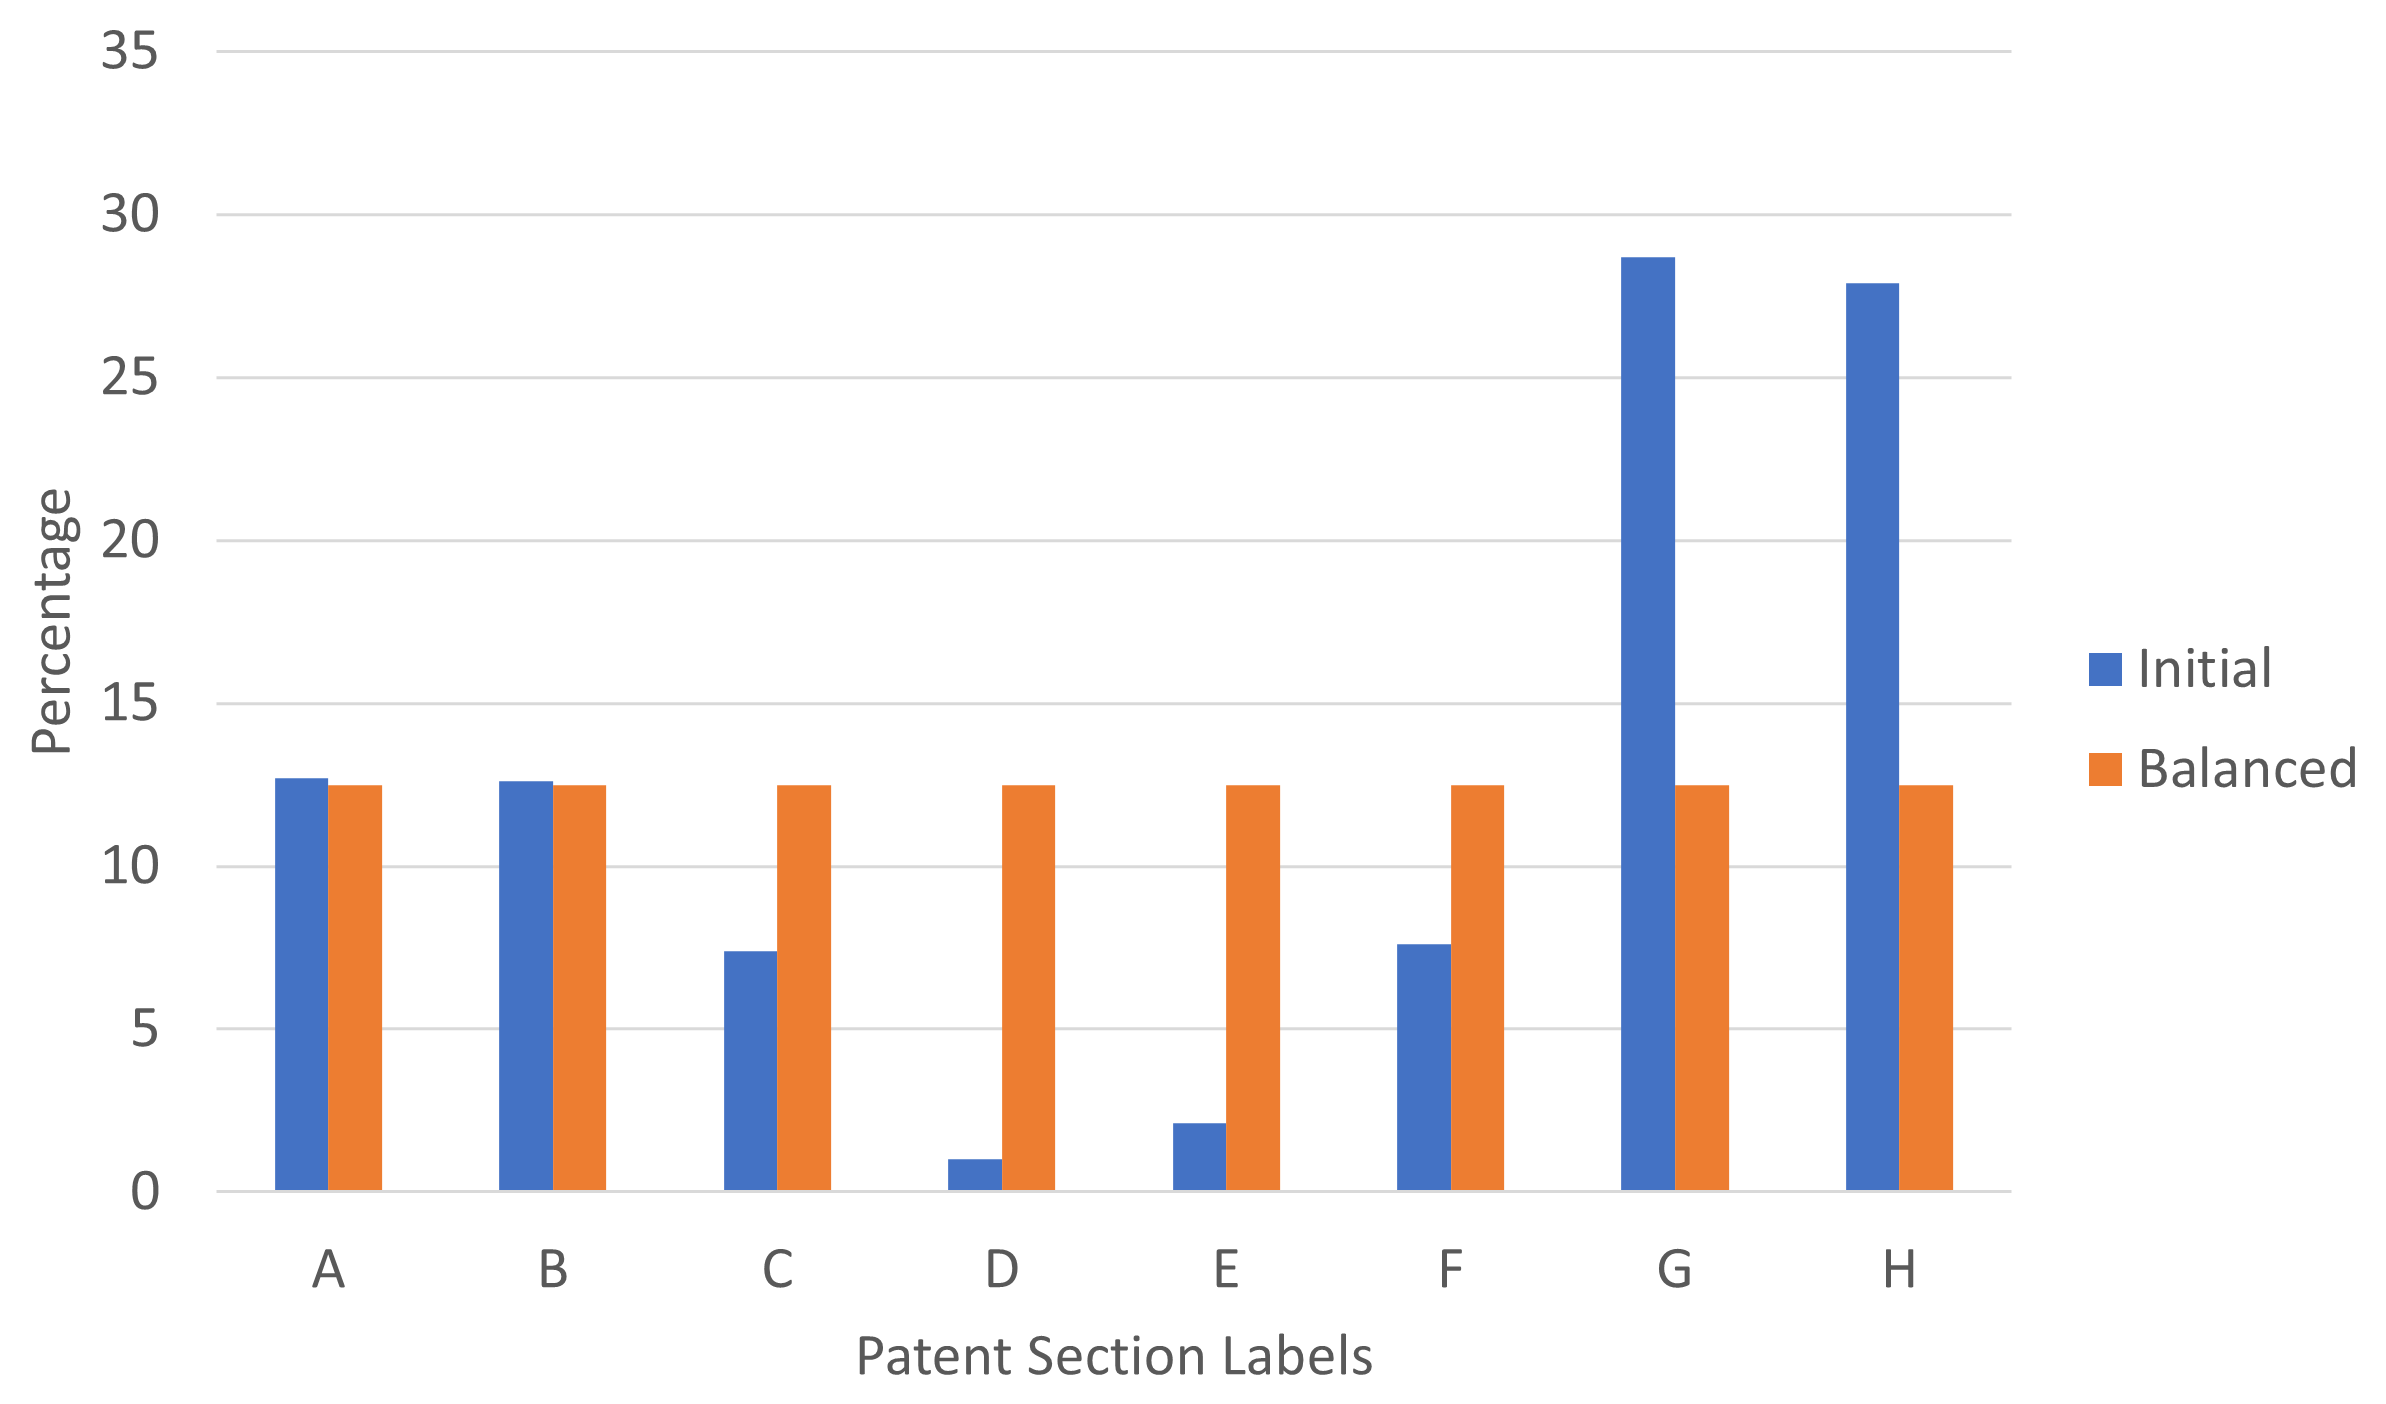
\includegraphics[width=14.5cm]{images/section_dist.png}
\caption{Patent document section balance}
\label{chart:section_dist}
\end{figure}

Ultimately, the Refined Patents dataset contains 200,000 patent documents, with each class having 25,000 documents and each document having a word count within the optimal bound. In Table \ref{tab:description_word_stats}, along with current document classification datasets, the presented dataset, namely, Refined Patents word statistics are provided. Contrary to unbounded word counts of the previous patent datasets that can fall even under only ten words for a document or go as high as a million words, the Refined Patents dataset sits in a more balanced bound of minimum and maximum word counts in a document.

Since word statistics are calculated using Python's NLTK (Natural Language Toolkit) tokenizer, which is a more human-readable tokenizer, the model varies slightly from the 512-4096 range resulting in the input stage. The reason why 512 was chosen as a lower limit is that this number is determined as the input limit in classical transformer architectures such as BERT. The Refined Patents dataset was prepared in this way to show the performance difference between classical approaches and the approaches of specialized transformers for long texts and to underline the advantage of these custom transformers. The upper limit of 4096 tokens is set as the maximum input limit even in custom transformer architectures such as BigBird and Longformer. An upper limit of 4096 tokens was applied to the dataset in order to always see the effect of changes to be made on these models on the full text, without the need for approaches such as trimming.

The most recent version of the dataset of this work can be found and downloaded publicly\footnote{https://huggingface.co/datasets/ufukhaman/uspto\_balanced\_200k\_ipc\_classification}.

\section{Patent Document Classification}

Automated patent document classification task holds critical importance for both the industry and academia (\citealt{task_CLEF-IP}). Firstly, the classification process is highly demanding labor performed by patent offices worldwide (\citealt{historical_patent_classification}). Even though there are already automated systems for patent classification, with an increasing number of patent applications (\citealt{DeepPatent}), improvements for automated patent classification systems are needed. Therefore, there have been several international open tasks for patent document data collection, classification, retrieval, and processing in general throughout the years. These are; Clef-IP tasks from 2009 to 2013: (\citealt{clef_ip_2009}, \citealt{clef_ip_2010}, \citealt{clef_ip_2011}, \citealt{clef_ip_2012}, \citealt{clef_ip_2013}), 2018 ALTA task (\citealt{task_ATLA_2018}) and finally NTCR patent tasks (\citealt{NTCIR_patent_tasks}). Results from most of these open tasks are collected and surveyed under the comprehensive works of \cite{patent_classification_book_survey} and \cite{patent_task_survey_2019}, presenting various ways to classify patent documents like heuristic approaches winnow (\citealt{lit_verbene_1}) and balanced winnow (\citealt{lit_beney_clef_ip_2010}), and GPLM which utilizes a relevance function between document class (\citealt{lit_aiolli}) showed in the Table \ref{tab:literature_results}.

% Please add the following required packages to your document preamble:
% \usepackage{booktabs}
\begin{table}
\centering
\begin{adjustbox}{width=\textwidth}
\begin{tabular}{@{}llllll@{}}
\toprule
Paper                       & Dataset         & Features                                         & IPC Level & Method                                                   & F1 Score \\ \midrule
\cite{Grawe-word-embedding} & USPTO & title and abstract                               & Section                  & LSTM                                                     & 0.63  \\
\cite{DeepPatent}           & USPTO-2M        & title, abstract                                  & Subclass                 & CNN                      & 0.40     \\
\cite{lit_aiolli}             & WIPO-alpha      & title, abstract & Subclass                 & GPLM             & 0.52     \\
\cite{lit_verbene_1}         & Clef-IP 2010    & abstract                                         & Subclass                 & Winnow                                                   & 0.56     \\
\cite{Lee-BERT}             & USPTO-3M        & title, abstract                                  & Subclass                 & Pretrained BERT                                          & 0.63     \\
\cite{lit_beney_clef_ip_2010}     & Clef-IP 2010    & title, abstract                           & Subclass                 & BalancedWinnow                                           & 0.68     \\
\cite{BigBird}              & USPTO-3M        & description                                  & Subclass                 & Tansformers (BigBird)                                    & 0.69

\end{tabular}
\end{adjustbox}
\caption{Patent classification results for different datasets and approaches}
\label{tab:literature_results}
\end{table}

As more semantic approaches have become widespread and proved to be competent in many areas, including text classification (\citealt{semantic_text_classification}), they have also started to be used in the patent document classification area. One of the first semantic text classification approaches that focuses on patents as long documents is the work of \cite{Grawe-word-embedding}, which uses an LSTM structure with word embeddings of patent document titles and abstracts from USPTO (United States Patent and Trademark Office) bulk data\footnote{https://bulkdata.uspto.gov/}, reporting 63\% F1 score for eight label classification task.

Another work, which again inputs only the title and abstract information of long documents from the data they also proposed (USPTO-2M\footnote{http://mleg.cse.sc.edu/DeepPatent/}) is DeepPatent (\citealt{DeepPatent}) which uses a CNN based approach with word embeddings for a similar but more challenging task being sub-class patent classification (638 multi-label classes) and reports an F1 score around 40\% (exact score is not specified in the paper). In continuation, the work of \cite{Lee-BERT} fine-tunes a pre-trained BERT (\citealt{BERT}) model for the same task with an expanded version of the USPTO-2M data being the USPTO-3M which is based on Google Patents Public Data\footnote{https://console.cloud.google.com/bigquery?p=patents-public-data\&project=articulate-run-341913} and reports a 63.74\% F1 score.

Improvement of transformer models such as BERT on long document classification tasks can be seen from this last example. However, it is still not competitive with evaluation scores of works such as \cite{single-label-BERT} and \cite{multi-label-BERT}, which address similar tasks with similar methods but for different datasets, containing less technical and shorter texts such as news reports. Even with cutting-edge methods like transformers, patent document classification remains a challenge. One possible reason for the hold-back is their inability to process long documents like patents within their parallel processing scheme.

Finally, Big Bird (\citealt{BigBird}) uses USPTO-3M data (\citealt{Lee-BERT}), which consists of 10,000 tokens per document on average for a patent classification task. The main difference of the Big Bird approach is that they have utilized not only the abstract or a part of the description text but the full description text up to 4096 tokens. This improvement in the input size was possible because of their new approach to classical transformers and as it can be seen, utilizing the full text, results in the highest performance compared to other studies.

\chapter{BACKGROUND}

Understanding the mechanisms behind transformers is crucial for understanding the idea of the thesis. Transformers (\citealt{attention_is_all_you_need}) are powerful structures for processing sequential data such as text. After each word of the text is tokenized under a certain vocabulary, pre-learned vector embeddings corresponding to these tokens substitute them. These token embeddings are calculated using the continuous skip-gram or bag-of-words methods suggested by \cite{word2vec}. In essence, these methods learn the correct mathematical representations of each word by vectorization  from large corpora of general use and minimize the cosine distance between neighboring vectors. These vectors are used in various tasks to replace words and represent their meanings. In the Transformers example, these learned vectors are used as an input for each token and the output can be the result of only one or all of these tokens. In the classification task examined in this study, a special token with its own vector is included to the beginning of the input text, and after an encoder process in which all other words contribute, the encoded version of this token is converted into classification probabilities with softmax. It consists of linear transformations made on these vectors based on the transformer structure. For the training phase, the result is back propagated using an appropriate loss function (cross entropy loss for the classification task) and the learnable parameters of the model are updated.

\begin{figure}[ht]
\centering
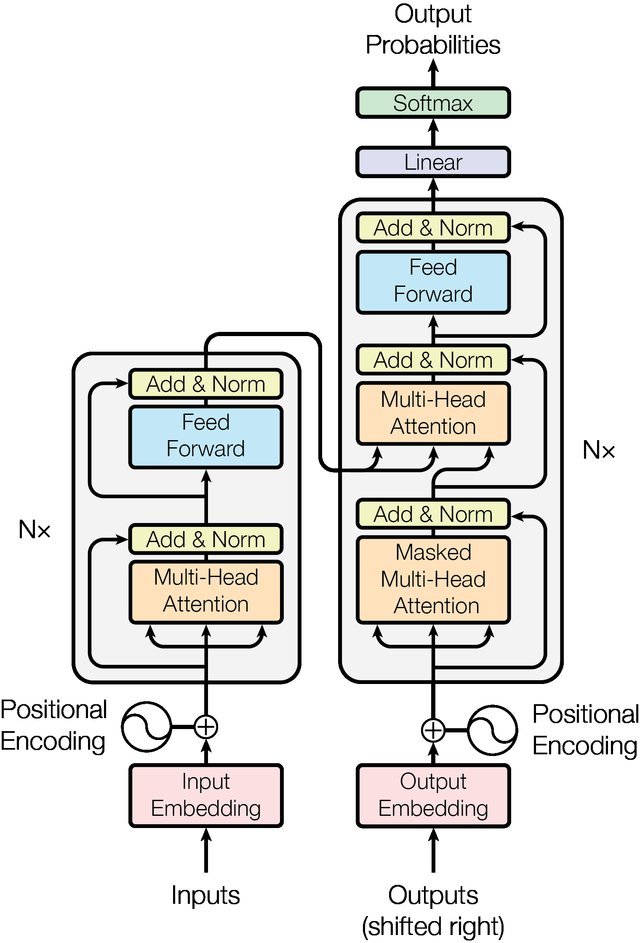
\includegraphics[width=10cm]{images/transformer_model_arc.jpg}
\caption{The transformer model architecture (Source: \cite{attention_is_all_you_need})}
\label{fig:transfomer_arc}
\end{figure}

Transformers perform the learning process through three essential matrices. These are matrices called query, key and value, which start with random value assignment and whose values are updated in each training cycle. These matrices have dimension \(n)\) as the input length and \(d\) as an arbitrarily chosen length, \((n,d)\). Each column of the query and key metrics, which are also a linear transformation of the input text, actually represents the values of an input token. Based on this, if the dot product of these two matrices is considered, the resulting output of this operation is a self-attention matrix, which will be interpreted as multiplying the embedding value of each token of the input text with all other tokens, including itself, i.e. associating it. Since the learnable parameter matrices are the same as the input size, for each newly added token, a new processing requirement occurs as long as the input text length, that is, the processing complexity is proportional to the matrix dimention \(d\) and the square of the input \(n)\). This causes transformers to have \(O(n^2d)\) computational complexity for n input tokens. This attention method, which is quite workable for text inputs that are not too long, becomes unmanageable due to quadratic coupling as the input length increases. A typical classical transformer architecture, including encoder and decoder structures, can be seen on Figure \ref{fig:transfomer_arc}.

In this chapter, firstly, their technical structure is introduced in their original form as \cite{attention_is_all_you_need} proposed. Secondly, their bottleneck, being a costly self-attention mechanism, which obligates computational limitations on the maximum possible input size to be processed in their single cycle, will be examined. Following, custom transformers, a version of transformers structured to cope with their self-attention bottleneck will be explained with different approaches. Methods of this thesis work are examinations and extensions on those custom or partial self-attention approaches.

\section{Transformers}

Transformers (\citealt{attention_is_all_you_need}) form the basis of widely used NLP models such as BERT (\citealt{BERT}), RoBERTa (\citealt{RoBERTa}), Pegasus (\citealt{Pegasus}), BART (\citealt{BART}) and XLNet (\citealt{XLNet}), which reported notable scores on NLP benchmarks including text classification task. They are briefly encoder-decoder structures (in some cases, they are only encoders like BERT, only decoders like XLNet, or utilize both like BART) with the self-attention mechanism forming their basis as a parallel process.

The encoder takes the learned word embeddings of the input sentence tokens at once. Since this is a parallel process, the encoder needs to add positional embeddings to differentiate the order of the input words, which is crucial for understanding a sentence's meaning. Position-aware input goes through two residually connected modules, a multi-head attention layer, and a fully connected feed-forward network, both followed by normalization modules. This process creates an embedding, representing the input sentence, or in this case, the input document (a collection of sentences, ultimately, a sequence of tokens).

For the task of sequence classification (just a generalized name for document classification), a special token ([CSL]) is inserted at the beginning of each data sequence, which is separated by a special separator token ([SEP]). The final embedding weight of the classification token determines the predicted class, and transformer dimensions should be adjusted accordingly such that the final output would result in a probability distribution vector of the size of the possible classes.

\begin{figure}[ht]
\centering
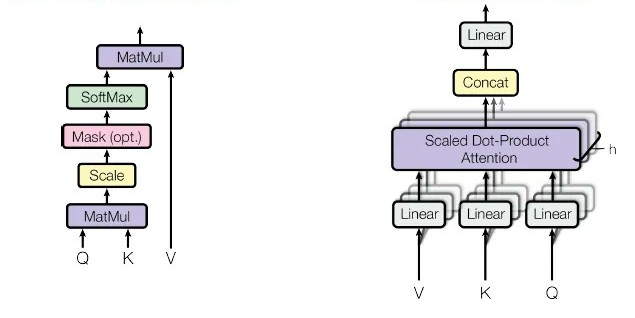
\includegraphics[width=15cm]{images/attention_details.jpg}
\caption{Scaled (left) and Multi-Head (right) attention schemes (Source: \cite{attention_is_all_you_need})}
\label{fig:attention_details}
\end{figure}

The decoder consists of a similar architecture to the encoder, outputting the next possible word, given the input words, using the power of various masked learning approaches. In order to perform sequence-to-sequence tasks, like translation, summarization, or question answering, the output of the encoder should be fed into the decoder for a sequence output. In other cases, the encoder output can be connected directly into a linear layer followed by a softmax operation to obtain the probability distribution, which is the working model of the document classification task.

\section{Attention Mechanism}

The attention mechanism is the heart of the transformers. It is the part where it is the most powerful but also the most costly. An attention function is basically composed of the dot product of the input embeddings' linear transformations. For simplicity, this process can be imagined as an input embedding matrix multiplied by itself. In detail, it is the softmax of the dot product of query matrix $XW_{Q}$ and the key matrix $XW_{K}$ where $X$ is the input embedding vector, $W_{Q}$ and $W_{K}$ are the learnable weight parameters that linearly transform the input embeddings, which formulated as in Equation \ref{eqSelfAttentionMatrix}.

\begin{equation}
\label{eqSelfAttentionMatrix}
QK^{T}=(XW_{Q}(XW_{K})^T)
\end{equation}

Obtained result $QK^{T}$ then scaled by $\sqrt{d_k}$ which is the square root of the dimension of the key matrix, goes through a softmax function and multiplies by the value matrix $V$, which is again a learnable parameter matrix and can also be shown as $XW_{V}$. Its final form is called scaled dot-product attention and formulated as in Equation \ref{scaled_dot_product_attention}. 

The formulation self-attention can also be represented within the transformer architecture with its multi-head structure, as on the right in Figure \ref{fig:attention_details}. In the multi-head structure, the processes shown in the formulation are processed multiple times in multiple layers and in parallel and used as a multi-dimensional matrix, allowing the model to focus on different features in different heads. Modern transformer architectures typically consist of 12 heads to provide a balanced structure to both provide model depth and prevent excessive complexity \cite{attention_is_all_you_need}. These different heads created are concatenated at the last stage by going through the same process. On the left side of Figure \ref{fig:attention_details}, the schema of the scaled dot product process represented in Equation \ref{scaled_dot_product_attention} is shown.

\begin{equation}
\label{scaled_dot_product_attention}
Attention(Q, K, V) = softmax(\frac{QK^T}{\sqrt{d_k}})V
\end{equation}

To sum it up, a matrix is created from the combination of each token of the input sequence, which is an embedding vector of a dimension \(d\), and the relationship, which is called attention, is calculated by the dot product of this matrix with another version of itself containing embeddings of the same input tokens, thus connecting each token of the input sequence with every token of the same input sequence. Consequently, for an input sequence with \(n\) tokens, the computational complexity for this attention operation would be equal to \(O(n^2d)\), creating a quadratic relationship between the model complexity and the sequence length while linearly related to the matrix dimension. This complexity comes from the $QK^{T}$ of the Equation \ref{eqSelfAttentionMatrix} and creates a severe bottleneck for the whole transformer process. A visual representation of this situation is shown in Figure \ref{chart:single_word_attention}

\begin{figure}[h]
\[\begin{tikzcd}[row sep=2.25em]
	Sunset & brings & a & sense & of & calm \\
	\\
	\\
	Sunset & brings & a & sense & of & calm
	\arrow[from=4-1, to=1-1]
	\arrow[from=4-1, to=1-2]
	\arrow[from=4-1, to=1-3]
	\arrow[from=4-1, to=1-4]
	\arrow[from=4-1, to=1-5]
	\arrow[from=4-1, to=1-6]
\end{tikzcd}\]
\caption{Single word full attention connection}
\label{chart:single_word_attention}
\end{figure}

Combined embedding vectors of words of the sentence 'Sunset brings a sense of calm' creates the input matrix. A single vector of this matrix, the embedding vector of the word 'Sunset' multiplied with every word embedding vector, resulting in \(n\) number of operations. This operation will be performed for every other word of the sentence (or, in full-scale document classification, for every word of the document). The critical point is that these are not series of vectors but matrices, and the dot product operation is performed at once for every word in a parallel fashion, creating an operation scheme and connections like in Figure \ref{chart:full_sentence_attention} where every word is attending to every word of the input sequence.

\begin{figure}[ht]
\[\begin{tikzcd}[row sep=2.25em]
	Sunset & brings & a & sense & of & calm \\
	\\
	\\
	Sunset & brings & a & sense & of & calm
	\arrow[from=4-1, to=1-1]
	\arrow[from=4-1, to=1-2]
	\arrow[from=4-1, to=1-3]
	\arrow[from=4-1, to=1-4]
	\arrow[from=4-1, to=1-5]
	\arrow[from=4-1, to=1-6]
	\arrow[from=4-2, to=1-1]
	\arrow[from=4-2, to=1-2]
	\arrow[from=4-2, to=1-3]
	\arrow[from=4-2, to=1-4]
	\arrow[from=4-2, to=1-5]
	\arrow[from=4-2, to=1-6]
	\arrow[from=4-3, to=1-1]
	\arrow[from=4-3, to=1-2]
	\arrow[from=4-3, to=1-3]
	\arrow[from=4-3, to=1-4]
	\arrow[from=4-3, to=1-5]
	\arrow[from=4-3, to=1-6]
	\arrow[from=4-4, to=1-1]
	\arrow[from=4-4, to=1-2]
	\arrow[from=4-4, to=1-3]
	\arrow[from=4-4, to=1-4]
	\arrow[from=4-4, to=1-5]
	\arrow[from=4-4, to=1-6]
	\arrow[from=4-5, to=1-1]
	\arrow[from=4-5, to=1-2]
	\arrow[from=4-5, to=1-3]
	\arrow[from=4-5, to=1-4]
	\arrow[from=4-5, to=1-5]
	\arrow[from=4-5, to=1-6]
	\arrow[from=4-6, to=1-1]
	\arrow[from=4-6, to=1-2]
	\arrow[from=4-6, to=1-3]
	\arrow[from=4-6, to=1-4]
	\arrow[from=4-6, to=1-5]
	\arrow[from=4-6, to=1-6]
\end{tikzcd}\]
\caption{Full attention connection of a sentence}
\label{chart:full_sentence_attention}
\end{figure}

The resulting scores are represented as a matrix of the attention scores of the word pairs. In classical approaches, this result would be a complete matrix, or in other words, a fully connected graph of word embedding relations. However, some recent works on transformers showed that the attention matrix is not necessary to be fully connected, but it can also be a sparse matrix containing up to 4096 word tokens, only not all of them attending every token of a long document, thus creating a custom attention mapping along the tokens of the document.

When a token attends all of the tokens, it is called a global token (\citealt{BigBird}); if it only attends a few, it is called a local token. Therefore, there can be custom attention mapping $A(X)$ consisting of both local and global tokens such that it is sparse enough to decrease \(n^2\) complexity but still dense enough not to reduce the performance of the transformer for the given task. The critical point, and the point this thesis investigates, is how to form this local attention mapping by deciding which tokens will be global or local, furthermore, how to choose which tokens a local token should attend to.

\section{TF-IDF (Term Frequency-Inverse Document Frequency)}

TF-IDF is the first of the methods proposed in this study to produce an alternative attention matrix. Although it has previously been used in various areas of natural language processing such as document clustering, the (\cite{tfidf}) transformer has not been used before to determine a custom attention mapping for the document classification task. TFIDF basically highlights the importance (distinctiveness) of words in a document and gives a score result for each document and each word of the document. In this study, these scores of the tokens of the input text (patent documents) were used as determining values in creating a custom attention mapping.

\begin{align} 
\label{tfidf}
	\begin{split}
		&\textrm{TF}(w_1) = \frac{\textrm{\# of $w_1$ in the document}}{\textrm{\# of words in the document}}\\ \\
		&\textrm{IDF}(w_1) = \log_2 \frac{\textrm{\# of documents}}{\textrm{\# of documents containing $w_1$}}\\ \\
        &\textrm{TF-IDF}(w_1) = \textrm{Tf} * \textrm{Idf}\\ \\
	\end{split}					
\end{align}

Scores are obtained by dividing the term frequency of words (or tokens in this case) by the inverse document frequency. As can be seen in Equation \ref{tfidf}, it focuses on how often the word \(w_1\) is used in a document and within documents in general. The number of times \(w_1\), which constitutes the numerator, appears in the document, underlines how important that word is for that document. More frequently used words are more important for that document. However, the point to be considered here is that although some stop-words (such as and and the) are used very frequently in texts, they do not actually contribute to the meaning of the content. The part that forms the denominator is there to prevent this situation. The denominator, which gives the number of occurrences of the word among all documents, decreases the TF-IDF score as it grows (that is, if the word is found in many documents). Meaning, words that are frequently found in a document but not in every document, and therefore words that play a distinctive role for that document, have a higher TF-IDF score. Considering a subject-based task such as patent document classification, input text contains technical terms and details, TF-IDF was used to select the words that have the potential to contribute the most to the attention matrix (by carrying the most distinctive information about the input) and therefore beneficial to be included in the custom attention mapping.

\section{PMI (Pointwise Mutual Information)}

\begin{equation}
\label{PMI}
\textrm{PMI}(w_1, w_2) = \log_2 \frac{P(w_1,w_2)}{P(w_1)P(w_2)}
\end{equation}

The other method recommended in this study to create custom attention mapping is PMI. As with TF-IDF, PMI, which is used in various areas of natural language processing (\cite{pmi}) and is especially powerful in evaluating pairwise connections, enabled the creation of custom attention mapping by scoring over token pairs. The dot product process, which produces the attention matrix, is performed on two matrices representing the input. Due to this operation, which means multiplying the transposed version of one of them, in this matrix multiplication, all words are actually connected to each other by multiplication with all other words.

As it is represented in the Figure \ref{chart:map_comparison}, the columns and rows represent each token, while the cells with connection points show the magnitude of the relationship between these two tokens. From this perspective, not only a token or word-based approach but also a token pair-based approach can be used. With the PMI scoring method, token pairs with high results are selected and these are used to create custom attention mapping. The equation is based on the probability of word-by-word pairs appearing together (how many times a given pair occurs relative to the total number of word pairs), as seen in ref{PMI}. In addition, the probabilities in the denominator are there to prevent tokens that may be too much as a pair, as they seem too much on their own. In this way, words that are frequently encountered in pairs but not so frequently individually become the word pairs with the highest PMI scores.

Considering the attention matrix within the Transformer structure, the data that constitutes the content of this matrix are actually the relationships of word pairs with each other. Therefore, the tokens included in the attention map process can be determined using PMI, which gives results based on the strength and distinctiveness of the pairwise connection of the token pairs.

Finally, PMI has a significant difference compared to TF-IDF. Since the number of occurrences of the token in the document is also a part of the formulation, TF-IDF actually gives the document-specific score of each token, that is, if the same token (word) is used again in different documents, these uses may have different scores. On the other hand, PMI performs statistical operations by combining all documents as a single large corpus and therefore reaches scores based on a vocabulary in which each word pair occurs once. A challenge caused by this difference is how far apart words will be considered as pairs. It is not necessary to accept only words that appear next to each other as pairs, in fact, this may cause some word pairs that may be interconnected with unrelated words but are actually related to each other to be overlooked. Instead, a window value \(w\) is determined and the word pairs within this window are considered as pairs, and the calculation can be performed on these pairs. The rest of the process continues by shifting this \(w\) window, which is determined to be 10 in this study, in a large corpus where all documents are combined.

\chapter{METHODOLOGY}

In order to overcome the input length limitation of the classical transformers, various new approaches were proposed. These approaches aim to decrease the quadratic complexity on the input size. One of the most preferred and promising methods to achieve the required efficiency is to sparse the attention matrix using custom attention mapping. By reducing and limiting the attention connections between input tokens, quadratic complexity can be decreased to a linear relation with the input size. However, there is a trade-off; reducing the attention connections imposes a risk of performance fall for the related model. Since transformers strongly rely on the attention mechanism for their success, finding and dropping only the most suitable attention connections is crucial while keeping as many valuable connections as possible. This thesis focuses on two prominent successful examples of work: Longformer, with its predetermined custom attention mapping, and Big Bird, with its combined predetermined and random attention mapping.

The project took the architectural baselines of both Longformer and Big Bird as a starting point for the experiments. Experiments with the different custom attention mappings are imposed over these architectures since they are already designed to work with custom attention mappings and are well suited to further customization. Along with two custom transformer architectures, a BERT model is utilized for the performance comparison of the classical transformer architecture on the refined patent dataset.

Two different local attention mapping approaches are controlled with both base architectures. These approaches are implemented in such a way that they replace the original process of these baseline models and run our custom local attention mapping algorithms instead. While keeping most of the other aspects of the architecture intact, Longformer and Big Bird models initiated with their pre-trained weights. Using pre-trained large language models and fine-tuning them for specific tasks with more domain-specific data became a universal approach for many NLP tasks (\citealt{pre_trained_models}). This approach utilizes pre-trained weights, which are obtained over extensive training cycles with general-purpose text data such as Books corpus (\citealt{books_data}) or Wikipedia articles and enable more independent researchers to work with models that have a general understanding of the natural language coming from billions of tokens. Moreover, a new classification head is applied with the required output dimensions for the patent document IPC classification task for both models.

Model parameters were decided with a random hyperparameter search method, using a search pool with values close to their original paper-presented parameters over a dedicated randomly sampled validation set of 1,000 patent documents. More detailed settings of the model parameters can be found in the model config files of the project GitHub repo\footnote{https://github.com/bekirufuk/long\_doc\_classification}.

A typical experiment is conducted after training with the refined patent dataset with the appropriate train and test data partitions. 20,000 and 3,200 randomly sampled disjoint patent document sets were used as train and test partitions. Models are always trained from their pre-trained base form for each distinct experiment, meaning that a cumulative training method has not been used. A typical train run has below main parameters, and again, more details on the training parameters can be found in the related config file of the GitHub repo. 

\begin{itemize}
  \item Epochs: 5
  \item Batch Size: 8
  \item Learning Rate: $3\times10^{-5}$
  \item Optimizer: AdamW
  \item Weight Decay: 0.01
  \item Warm-up Rate: 0.1
  \item Scheduler Type: Cosine
\end{itemize}


\section{Preprocessing}

For the data prepossessing, the project followed the action points:

\begin{enumerate}
   \item Granted patent documents from the years between 1990-2020 in the USPTO's database of approved patents have been downloaded and organized as a separate table for each year from the public resource.
   \item The dataset, which contains the class information, was first mapped as a single table, and for all records, three levels of IPC information (sections, Class, Subclass), unique patent code, title, abstract, and detailed explanation (main text) merged into a single table format.
   \item Records that are..
       \begin{enumerate}
           \item Blank or unreadable text content in the detailed description section
           \item Duplicated patent code
           \item Missing classification information
           \item Outside of the standard 8 IPC sections (0.01\% of data classified with unofficial notations)
      \end{enumerate}
        .. were excluded.
   \item Non-UTF-8 characters removed from all documents (causes errors in the tokenization process)
   \item Existence of stop-words empirically controlled with several train and test runs. Removed since it caused no difference in the final results. Their removal provides an 8\% performance gain on operation speed. (word statistics represent excluded version)
   \item Patent documents filtered by their word counts (510($<$)length$<$)4094). Words were counted using an NLTK (Natural Language Tool Kit) tokenizer instead of a more specific one like BERT or Longformer pretrained tokenizer in order to achieve a more general representation of document length filtering. All word statistics are calculated by NLTK word tokenizer.
   \item Patent documents further filtered for class balancing. Random n documents were selected for each IPC section, n being the record count for the section with the least amount of data, resulting in 25,000 patent documents for each section. Thus, the final dataset contains 200,000 refined patent documents.
 \end{enumerate}

\section{Tokenization}

Like large language models, tokenizers can also be pre-trained and served along with their models. All three transformer models utilized for this project have their own distinct features in terms of tokens. They have particular token IDs and special token representations. Thus, these conventions should always suit the data to obtain correct results. Therefore, as a tokenizer, each model's own pre-trained tokenizer is used to get the tokens, creating three tokenized versions of the patent data.

On the other hand, an independent BERT-based tokenizer was also trained for the utilized tokenization process. However, test accuracy results were down 10\% compared to when a dedicated tokenizer was used. Thus, each model's specific pre-trained tokenizer is used instead of a trained universal tokenizer.

Pre-trained tokenizer parameters may cause nuance differences within themselves, which may lead to dissimilarities in the tokenization of words. For example, while the tokenizer of the Longormer model processes a word such as "reconstruct" as a single token, the tokenizer of the Big Bird model may choose to separate this word into two tokens, "re" and "construct". The source of such a preference is, of course, related to the characteristics of the dataset on which these tokenizers were trained.

Although both tokenizers have similar operating principles, Big Bird uses a tokenizer based on Sentencepiece (\cite{sentencepiece}), while Longformer uses a tokenizer based on RoBERTa (\cite{RoBERTa}). This difference in nuance was another reason why these models utilized with their own specially trained tokenizers, rather than running them on a common tokenizer.

The use of tokenizer plays a critical role in preparing the dataset for training, as well as determining the TF-IDF and PMI scores that will be used to determine custom attention mapping. These scores, which will determine whether the relevant token will be included in the self-attention process or not, each belong to a token, not a word.

\section{Limitations}

Working with transformers, especially processing and experimenting on cutting-edge input limits like 4096 tokens, requires an extensive amount of computing power, even with efficient methods. For an Nvidia GPU with 12GB dedicated memory, training can only be performed with batches of 8, which, along with the model parameters, fully utilizes the available GPU. An entire train-test run of the collected dataset of 200,000 patent documents would take approximately 120 hours with this project's best available technical capabilities. In order to increase experiment counts and obtain a more agile process, experiments are scaled down to 20,000 patent documents for training, which takes 12 hours on average to run, creating not a performative but an agile, comparative ground base for a total of 40 experiments with various models and local attention mapping settings.

\section{Custom Local Attention Mappings}

\begin{figure}[ht]
\centering
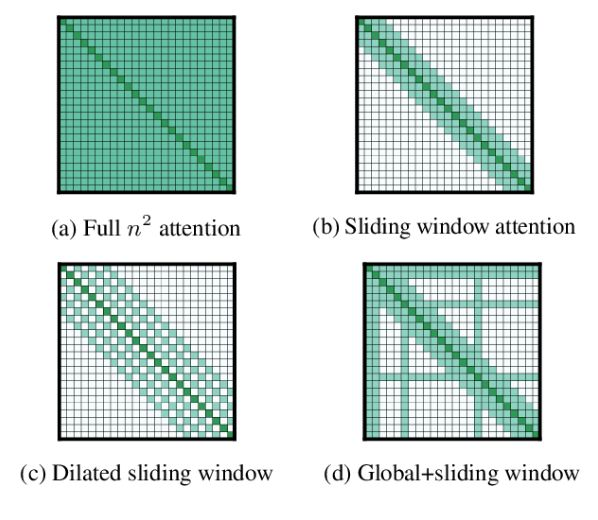
\includegraphics[width=12cm]{images/attention_comparison.jpg}
\caption{Attention mapping visualisations of Longformer (Source: \cite{longformer}}
\label{chart:map_comparison}
\end{figure}

While there are various approaches to creating a custom local attention mapping, the most common methods that BirBird and Longformer utilize are pre-defined and random approaches. However, there is no application of a statistical approach to create attention mapping, as an extensive literature review suggests. Different tokens of the input text hold different information values to the whole document, which might indicate whether the token should be included or omitted in the attention score calculation process. Ultimately, none of the tokens will be omitted entirely from the process since locally connected tokens create an information chain that can be carried over between non-directly connected tokens. In this sense, efficient local attention mapping methods mimic the behavior of a CNN (Convolutional Neural Network) compared to a fully connected network. Instead of globally connecting each token to each, they specify only certain token connections that exist in a local window. \cite{longformer} represents these connections as colorings in a 2D matrix. Illustrations from their paper can be seen in Figure \ref{chart:map_comparison}. Part (b) represents the scenario where a token only attends to itself and neighboring certain tokens. Besides, different connection patterns can be used, as shown in part (c). Finally, their mapping proposal is represented in part (d). A similar coloring pattern can also be observed in BirBird, the only difference being that global connections are not predetermined but consist of randomly selected blocks of 64 by 64 tokens.

\begin{figure}[h]
    \centering
    \begin{subfigure}[b]{0.49\textwidth}
        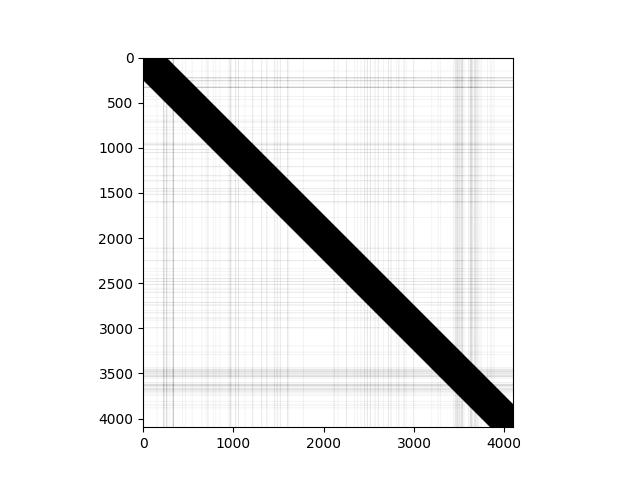
\includegraphics[width=1\textwidth]{images/0_local_and_tfidf.jpg}
        \caption{}
        \label{fig:tfidf_mapping1}
    \end{subfigure}
    
    \begin{subfigure}[b]{0.49\textwidth}
        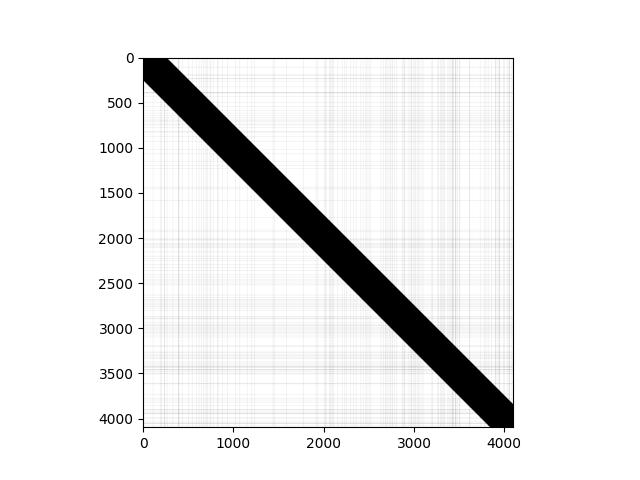
\includegraphics[width=1\textwidth]{images/1_local_and_tfidf.jpg}
        \caption{}
        \label{fig:tfidf_mapping2}
    \end{subfigure}
    \hfill %add desired spacing between images, e. g. ~, \quad, \qquad, \hfill etc. 
      %(or a blank line to force the subfigure onto a new line)
    \begin{subfigure}[b]{0.49\textwidth}
        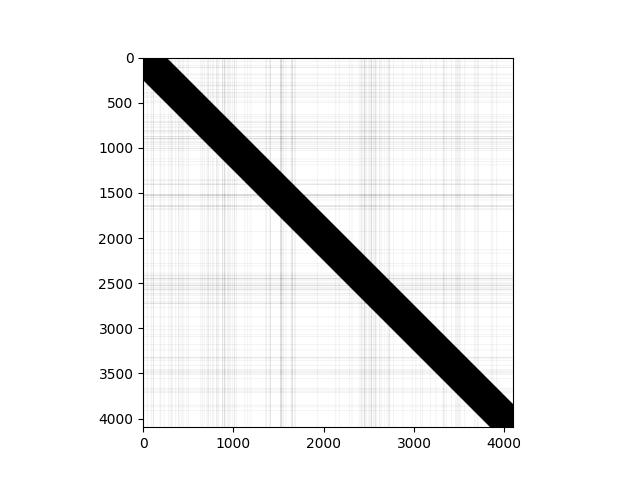
\includegraphics[width=1\textwidth]{images/4_local_and_tfidf.jpg}
        \caption{}
        \label{fig:tfidf_mapping3}
    \end{subfigure}
\caption{Local window and TF-IDF based attention mapping examples from patent documents}
\label{fig:custom_mapping_examples}
\end{figure}

In addition, we present not a representative but the actual attention mappings obtained from the Longformer model using local window and TF-IDF based calculations in Figure \ref{fig:custom_mapping_examples}. Each coordinate point on these maps represents a dual token relation, the x and y coordinates being the tokens of a patent document of approximately 4096 tokens; darker points indicate an attendance of that token relation to the self-attention process. While the vertical and horizontal mild lines represent statistically chosen 128 global tokens, the diagonal bold line represents the sliding local attention window connections of 512 tokens (256 tokens from left and right) for each token. As seen in examples a, b, and c of Figure \ref{fig:custom_mapping_examples}, the TF-IDF approach focuses on different parts (or uniformly focus) of the input for different documents in a context-aware fashion.

To sum up, two main statistical approaches were tested for creating a custom local attention mapping that scales down and approximates the full self-attention mechanism: TF-IDF and PMI. Each token (or token pair) has a calculated TF-IDF or PMI score, and 128 tokens with the highest score are selected to be global tokens, connecting to all of the tokens due to their statistical significance in the context of the given document. Thus, creating a custom local attention mapping pattern, which will be injected into the vanilla architecture of the transformer models Longformer and BirBird, instead of their attention mapping pattern, will ultimately be used to calculate the self-attention scores.

\subsection{TF-IDF Mapping}

To obtain TF-IDF scores, the formula shown in Equation \ref{tfidf} was applied for each token on the tokenized versions of all patent documents to be used in the training phase. This operation produced a score for all tokens for each document. The obtained scores were saved in a dictionary as a local file to be used during the training phase. During the training, for each input that came in batches of 8, the relevant TF-IDF scores were read from the dictionary, again in batches of 8. For each document, the position indexes in the input matrices of the 128 tokens with the highest score among the scores of all the tokens in the document were choosen and custom local attention mapping completed with the sliding attention connections. The created custom attention mapping reduces the complexity of the model from \(O(n^2d)\) to \(O(nd)\) because now, as the input size increases, the only thing that will get longer is the window attention structure passing through the diagonal, which is the same for each new one. For the token, it increases by a fixed number (by the window width), not by the input length. Therefore, complexity has a linear relationship with the length of the input and the size of the parameter matrix. In addition, the number of global tokens determined does not change and remains constant regardless of the entry length.

\subsection{PMI Mapping}

A similar method to TF-IDF was followed in calculating and using PMI scores. Scores are calculated for each word across all documents, as shown in Equation \ref{PMI}. Unlike TF-IDF, there is a single score for a word pair that can be seen anywhere, rather than separately for the same words in different documents, and is recorded in a local dictionary in this way. In this study, all words falling within the range of 10, which is the window variable determined, are considered to be pairs with each other and word pairs are determined in this way. While determining the pairs within the window range, the order of the words is not changed, that is, the symmetrical versions of the word pairs are not added to the dictionary. Such a situation can only happen if the symmetric version of that pair appears elsewhere in the corpus within the same window as that order. After the scores of all detected word pairs are recorded in a dictionary, just like in TF-IDF, the documents are put into the training cycle in batches of 8 and a selection is made based on the PMI scores of the word pairs of the relevant documents corresponding to the dictionary. Since the words are selected as pairs, in order to keep the number of global tokens constant between experiments, 64 token pairs with the highest PMI score (128 tokens in total) are selected and the positions of these tokens on the input matrix are combined with sliding window attentions to create a custom local attention mapping.

\section{Control Attention Mappings}

Along with the two statistical approaches and pre-trained models' default (vanilla) forms, two extra custom attention mapping methods were tested as a base and trivial examples.

In addition to statistical custom attention mapping (TF-IDF and PMI), two basic structures consisting of simpler rules were tested in the same way. These custom attention changes are replaced with the models' default attention mapping just before the attention matrix is created within the model's pipeline. However, it is necessary to check whether this change really has a positive or negative effect with another mapping method. For this process, two trivial mapping methods were chosen: random attention mapping and first n attention mapping. Compared to past studies or the statistical methods in this study, these two mapping methods are basic approaches that do not focus enough on the necessary attention connections, are completely independent of the content, and only show whether the model bases work properly with custom mapping structures, and finally, they also shows that if an inadequate mapping method is used, the performance will actually be affected negatively as accuracy scores on Figure \ref{chart:accuracy_result} shows.

\subsection{Random Attention Mapping}

Random attention mapping is the process of selecting global tokens that will enter the self-attention process only randomly. Out of all the tokens on the document, 128 are randomly selected and this pattern creates the custom local attention mapping pattern. All other operations performed after the random pattern is formed proceed in the same way as in TF-IDF and PMI mappings.

Random attention mapping differs from Big Bird's random block attention, which does not select individual random tokens but random areas throughout the document, representing 64$x$64 block in a 2D attention matrix. Big Bird also uses randomness in its attention mapping structure and determines the global tokens randomly. However, Big Bird's randomness approach is different from the random control attention mapping approach because Big Bird works on random token blocks, not random tokens. These token blocks consist of 64 adjacent tokens and their corresponding columns and rows, that is, 64x64 blocks. What is determined randomly in a Big Bird structure is the position of these blocks. For this reason, the one used here is not a simple attention mapping method, but an approach that aims to add randomness to the process by continuing to keep tokens that are close to each other together. Random attention mapping, on the other hand, is based solely on the individual random selection and use of global tokens.

\subsection{First n Tokens Attention Mapping}

In addition to random attention mapping, another method used for control mapping in simple custom local attention mappings is to directly take the first n tokens globally. Again, as in other mapping structures, a total of 128 tokens were selected, that is, the first 128 tokens of the document are determined globally and used together with sliding window attentions in the attention matrix calculation. The method of selecting the first n tokens reflects the classical transformer working mechanism, which before specialized transformer structures for processing long texts could not process more than 512 tokens. For example, if you want to work on a text that exceeds the input limit with BERT, the simplest and fastest way is to trim the tokens behind the limit, that is, to accept only the first n tokens as in this experiment. Certainly, in this custom local attention mapping, tokens outside the first 128 are not excluded from the process, they are not just determined as a global token, they add their semantic layers to the final attention matrix that emerges by being gradually connected to each other with sliding window attention.

\chapter{RESULTS}

Longformer and Big Bird models, which were made suitable for working with custom local attention mappings, were subjected to a single classification task consisting of 8 options, at the IPC (International Patent Classification) section level, on the Refined Patents dataset. First of all, the Longformer and Big Bird models, both vanilla (default) versions and versions with TF-IDF and PMI custom attention mappings, were tested on the same data set. This test pattern produces 6 results in total. In addition, when the control attention mapping methods random attention mapping and first n attention mapping are added, we obtain 10 results in total, 5 for each model. Finally, in addition to BERT, which is a classical transformer approach, and transformer structures, results were also presented for comparison with Naive Bayes and SVM methods, which are among the basic methods that can be used in the document classification task. Results from the experiments collected under ten main accuracy scores are shown in the Figure \ref{chart:accuracy_result}

\begin{figure}[ht]
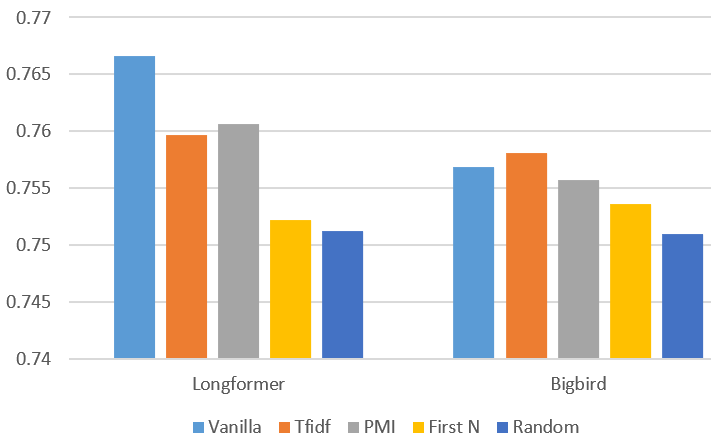
\includegraphics[width=15cm]{images/accuracy.png}
\caption{Accuracy scores for Refined Patents with both models under different local attention mappings}
\label{chart:accuracy_result}
\end{figure}

The results show that the statistical token selection method TF-IDF slightly improves Big Bird accuracy scores, which is not true for Longformer, resulting in a $76\%$ accuracy score. Although the accuracy differences are not statistically significant and score changes within a $\pm 0.5\%$ bound, the statistical attention mappings work better than the random and first n approaches by a margin of $1\%$ in the case of Longformer. The default Longformer method, which uses a local sliding window attention mapping along with a predetermined global token selection, still performs the best compared to statistical approaches; however, TF-IDF and PMI methods do not significantly decrease the performance either. On the other hand, trivial control experiments first n and random fall behind with a larger margin, showing the effect of employing different approaches over trivial methods. For the case of Big Bird, scores are more uniformly distributed, favoring the TF-IDF approach over all others; however, the score difference is not significant enough to establish a notable performance increase yet, comparing equal with the original approach, which indicates a possibility of new applications for the statistical point of view to the local attention mappings.

Apart from the accuracy scores presented in Figure \ref{chart:accuracy_result}, the same dataset was also evaluated with more traditional methods. Figure \ref{chart:classical_eval} shows the best performing classical model as BERT with a $72\%$ accuracy, which falls behind the more modern approaches specifically tailored to work with long text documents as expected. Similarly, SVM with $70\%$ and Naive Bayes with $60\%$ classification accuracy scores again show the improvement of modern NLP methods in the example of a long document classification task. However, even if it provides an improvement over older methods, it lags behind classical transformers such as BERT, especially when working on word-length content that exceeds the input size. This is one of the main reasons for the emergence of transformers such as Longformer. When we look at the previous studies on transformers, especially since they work with serial logic rather than parallel, as the input length increases, they fall significantly behind in evaluating the information spread throughout the document when they need to make a prediction for a task such as keeping historical information cumulatively and classification.

\begin{figure}[ht]
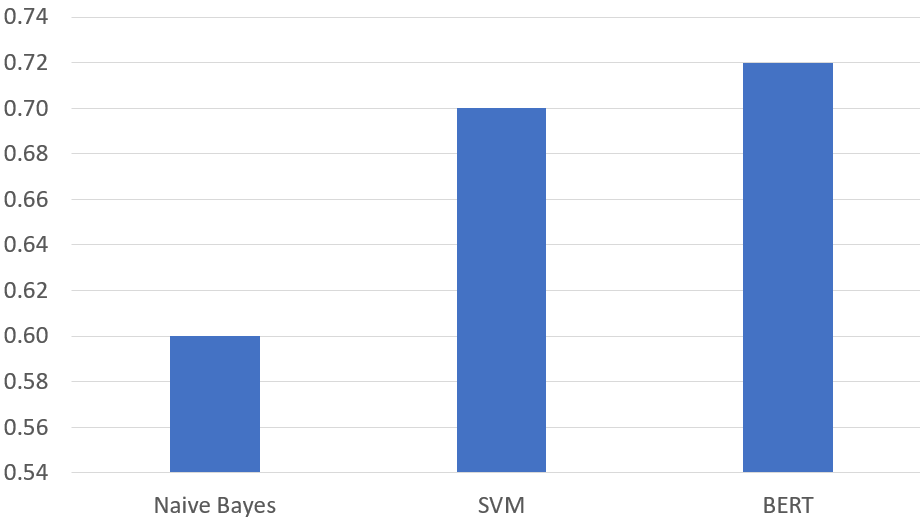
\includegraphics[width=15cm]{images/classical_eval2.png}
\caption{Classification accuracy scores for Refined Patents with classical approaches}
\label{chart:classical_eval}
\end{figure}

\section{Classification Details}

The models used in this study attempt to assign patent documents to one of the 8 classes that appear in Table \ref{tab:ipc_sections}. These 8 classes are the sections that the IPC determines as the outermost classification level and are used to create an entry-level distinction, a taxonomy, on patent documents. While there are relatively more unique classification options from the IPC section values such as "Human Necessities", "Fixed Constructions" or "Chemistry", on the contrary, there are also options such as "Physics" and "Electricity", which are close to each other in subject meaning despite being the main classification level. available. Since electricity is also a physics subject, these two topics may seem difficult to separate from each other.

Figure \ref{chart:confusion_matrix}, shows the classification results of the Longformer model in vanilla form. In this figure prepared in a confusion matrix format, the letter values corresponding to the descriptions of the IPC sections can be seen at the x and y dimensions. Descriptions of these values are available in Table \ref{tab:ipc_sections}. While there are actual IPC section values in the y dimension on the confusion matrix, the predictions of the model are in the x dimension. When viewed this way, the percentage value in each cell shows the accuracy specific to that IPC section. This means that values outside the diagonal line indicate incorrectly predicted classes, and what their correct values should be. Of the cells outside the diagonal, the most prominent are the opposite cells of categories G and H. Looking at these cells, it can be seen that about 11\% of the patent documents that should have been H were incorrectly predicted as G. Likewise, about 15\% of patent documents that should have been G were incorrectly predicted to be in H class. Considering that class G is physics and class H is electricity, it can be seen that the complex structure of these subjects, which are very close to each other, is also reflected in the model predictions.

When other cells outside the diagonal are examined, classes that the model incorrectly predicts stand out, but none of them come to the level of confusion between the physics and electricity classes with values of 11% and 15%.

\begin{figure}[ht]
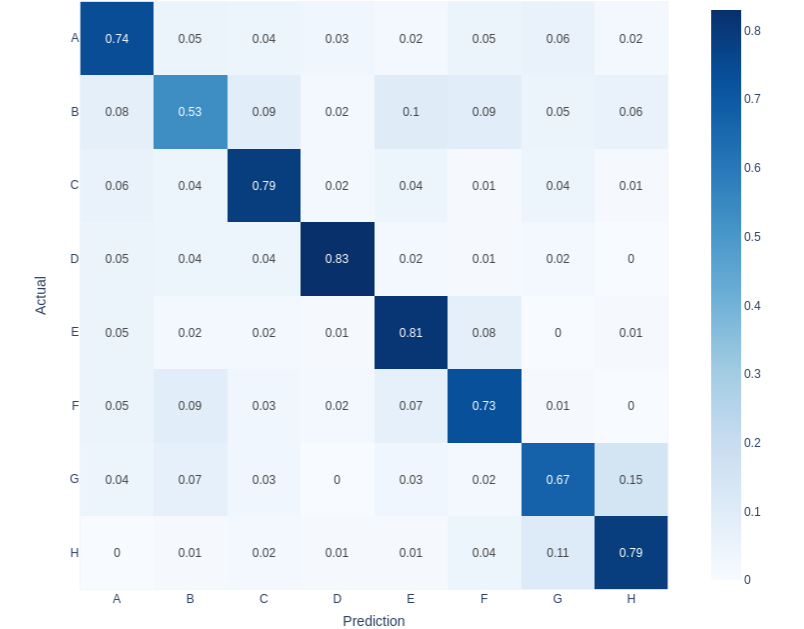
\includegraphics[width=14.5cm]{images/confusion_matrix.png}
\caption{Patent documents classification details}
\label{chart:confusion_matrix}
\end{figure}

\section{Qualitative Analysis}

In order to investigate the effects of a statistical approach, a qualitative analysis was performed for the TF-IDF local attention mapping method using the Longformer model as a testing ground. Table \ref{tab:qual_analysis} shows the top selected words for an example of a patent document from each class.

\begin{table}[ht]
\centering
\begin{tabular}{ll}

Patent Class                                & Tf-Idf Selected Words        \\ \hline
\multicolumn{1}{l|}{Electricity}            & power, telephone, signal     \\
\multicolumn{1}{l|}{Fixed Constructions}    & housing, lever, latch        \\
\multicolumn{1}{l|}{Chemistry}              & dissolves, solvent, reaction \\
\multicolumn{1}{l|}{Physics}                & conductive, signals, analog  \\
\multicolumn{1}{l|}{Performing Operations}  & trimming, assembly, shaft    \\
\multicolumn{1}{l|}{Human Necessities}      & tape, supplies, buttons      \\
\multicolumn{1}{l|}{Textiles}               & fibre, layer, polyurethane   \\
\multicolumn{1}{l|}{Mechanical Engineering} & mechanism, heat, liquid     
\end{tabular}
\caption{TF-IDF selected words for patent classes}
\label{tab:qual_analysis}
\end{table}

Upon investigation of the words, it can be seen that the words that yield the highest TF-IDF score -therefore selected as global tokens to attend the self-attention operation- are the words that can be in a way related to the corresponding actual class of the patent document. From this point of view, the TF-IDF approach is an effective way of creating a custom local attention mapping since it can focus on related words and even be informative about the actual class of the document. However, this notion does not directly reflect on the accuracy scores.

Finally, the results of the qualitative analysis appear to be in agreement with the results in Figure \ref{chart:confusion_matrix}. While the most confused classes in the confusion matrix are electricity and physics classes, Table \ref{tab:qual_analysis} shows the distinguishing words determined by TF-IDF in physics and electricity classes and indicates the words "signal/signals" for both classes. In other words, there is a connection between the similarity of TF-IDF words between these two classes and the similarity of the classification results.

\chapter{CONCLUSION}

The long document classification task is one of the most challenging text classification tasks. In addition, patent documents are complex, structurally profound, and have a wide range of technical vocabulary, making them not trivial data to work on. The combination of these two areas creates a remarkably challenging environment. Of course, past studies have stretched and improved the available utilities to achieve the highest possible performance by using state-of-the-art structures for a challenging environment like this. Transformers are robust, powerful, and flexible models that have proven themselves in many areas and produced pioneering results in various tasks. However, a relatively new implementation version of transformers, specialized for working on long, sequential inputs, is only being deepened and getting more comprehensive with each influential work. It is a rich and growing field with the potential to contain many undiscovered methods to experiment with and obtain interesting results using various custom local attention mappings.

Custom local attention mappings portray a recipe for an efficient calculation of the self-attention matrix, reducing the quadratic relation between input length and required memory space to linear, thus allowing input lengths up to 4096 tokens to be processed parallelly, which was not possible with classical transformer architectures. 

In this thesis study, two approaches to these methods were tested and evaluated for their effects on the long document classification task with the Refined Patents dataset, using two acknowledged custom transformer architectures as base models.

Presented Refined Patents dataset, arranged specifically for the long document classification task, containing only detailed description sections of documents that are challenging in length to the classical transformer structures, as a class-balanced collection of 200,000 preprocessed and cleaned USPTO (United States Patent and Trademark Office) granted patent documents in English from the last 30 years along with their IPC classification information to the sub-class depth.

Longformer and Big Bird pre-trained transformer models were utilized, fined-tuned, and tested with the Refined Patents dataset in order to observe the effects of the statistical custom local attention mappings constructed with TF-IDF and PMI scores of the input document tokens.
 
According to accuracy results, one method does not significantly surpass the other. However, both statistical methods examined are functional and effective methods that can sparse the self-attention matrix while preserving the initial performance of the models, providing a possible alternative method for an efficient transformer strategy. Furthermore, qualitative analysis shows that TF-IDF is capable of pointing out statistically significant words within a patent document that also appear as relative terminology to the class of the document.

The words resulting from TF-IDF scores from the Table \ref{tab:qual_analysis} is also in agreement with the uncertainties on the confusion matrix shown in Figure \ref{chart:confusion_matrix}. Accuracy results from this work and also other reporting previous works that are listed in the Table \ref{tab:literature_results} show that transformer models are successful in patent document classification task, one of the most challenging tasks of document classification, they show higher performance against non-transformer-based approaches like Naive Bayes, SVM, CNN or LSTMs. Input length seems to be one of the most important problems for transformers to achieve the highest success and find meaning in long inputs and use it in tasks such as text generation or classification. As the text becomes longer, it becomes more difficult to process the entire input and therefore find the meaning scattered throughout the text. Increasing the input limit of transformers and enabling them to process longer textual data with methods such as custom attention mapping significantly increases their success. However, it seems that simply using different mapping methods does not cause an increase on the performance necessarily. This is mainly due to the robust structure of transformer models and their ability to show high success in challenging tasks, even in their straightforward forms.

Although the proposed statistical methods, TF-IDF and PMI, to create a custom local attention mapping did not provide a direct increase in the operating performance of the transformer model, they did demonstrate the usability of an alternative approach method to efficient transformers. Statistical approaches are also an option for transformers that are tried to be effective on long inputs with various methods, from learnable methods to randomness, and it is possible to exceed their current performance with future improvements on these statistical methods. Dahası, sınıflandırılmaya çalışılan IPC seviyesi derinleşebilir ve sadece section bazında değil de, class hatta sub-class bazında sınıflandırma çalışmaları için de kullanılabilirler.

\bibliographystyle{ACM-Reference-Format}
\bibliography{main}

\end{document}